% introducao
\chapter{Introdução}
No início dos tempos, Donald E. Knuth criou o \TeX. Algum tempo depois, Leslie Lamport criou o \LaTeX. Graças a eles, não somos obrigados a usar o Word nem o StarOffice.

\section{Figuras e tabelas}
Esta seção faz referência às Figuras~\ref{fig:ex1} e~\ref{fig:ex2}, a título de exemplo. A primeira representa o caso mais comum, onde a figura propriamente dita é importada de um arquivo \texttt{.eps} (aplicativos como \emph{xfig} e \emph{dia} estão entre os mais usados para gerar figuras no formato \texttt{.eps}). A segunda exemplifica o uso do environment \texttt{picture}, para desenhar usando o próprio~\LaTeX.

\begin{figure}
        \centerline{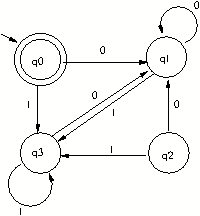
\includegraphics[width=8em]{images/fig.png}}
        \caption{Exemplo de figura importada de um arquivo \texttt{.eps} e também exemplo de caption muito grande que ocupa mais de uma linha na Lista de~Figuras}
        \label{fig:ex1}
\end{figure}

% o `[h]' abaixo é um parâmetro opcional que sugere que o LaTeX coloque a
% figura exatamente neste ponto do texto. Somente preocupe-se com esse tipo
% de formatação quando o texto estiver completamente pronto (uma frase a mais
% pode fazer o LaTeX mudar completamente de idéia sobre onde colocar as
% figuras e tabelas)
%\begin{figure}[h]
\begin{figure}
        \begin{center}
        \setlength{\unitlength}{.1em}
        \begin{picture}(100,100)
                \put(20,20){\circle{20}}
                \put(20,20){\small\makebox(0,0){a}}
                \put(80,80){\circle{20}}
                \put(80,80){\small\makebox(0,0){b}}
                \put(28,28){\vector(1,1){44}}
        \end{picture}
        \end{center}
        \caption{Exemplo de figura desenhada com o environment \texttt{picture}.}
        \label{fig:ex2}
\end{figure}

Tabelas são construídas com praticamente os mesmos comandos. Lembre-se, porém, que o caption das tabelas deve ir em cima.

\subsection{Classificação dos etc.}

O formato adotado pela ABNT prevê apenas três níveis (capítulo, seção e subseção). Assim, \texttt{\char'134subsubsection} não é aconselhado.

\section{Sobre as referências bibliográficas}
Recomenda-se seriamente fazer uso do pacote \emph{bibabnt}, também disponibilizado na página do UTUG~\citeyearpar{UTUG:Homepage-01}. Esse pacote provê um estilo \textsc{BibTeX} para formatação de referências bibliográficas combinando normas da ABNT e do Instituto de Informática da UFRGS\@.

As seguintes referências são colocadas aqui a título de exemplo:
\cite{Andrews:CP-91, Silberschatz:OSC-3-91, Wilson:MME-01}.

A classe \emph{iiufrgs} faz uso do pacote \emph{natbib}. Esse pacote
disponibiliza diversos comandos alternativos para
citações. Os mais úteis para nós são o \texttt{\char'134citeyearpar},
que produz somente o ano (ex.~``[\ldots] são apresentados por Baker e
Smith~\citeyearpar{Baker:PP-96}.'') e o
\texttt{\char'134citep*}, que produz a citação com a lista
completa de autores (ex.~``[\ldots] na linguagem Panda~\citep*{Assenmacher:Panda-ECOOP93}.'')
